\documentclass[unknownkeysallowed]{beamer}
\usepackage[french,english]{babel}
\usepackage{../sty/beamer_js}
\usepackage{../sty/shortcuts_js}

\usepackage{dirtree}
\newcommand{\Benchopt}{\texttt{Benchopt}}

\definecolor{tomcolor}{rgb}{0.,.3,.6}
\lstset{basicstyle=\color{tomcolor}\scriptsize\ttfamily}
\addbibresource{../biblio/biblio.bib}
\captionsetup[subfigure]{labelformat=empty}
\begin{document}

%%%%%%%%%%%%%%%%%%%%%%%%%%%%%%%%%%%%%%%%%%%%%%%%%%%%%%%%%%%%%%%%%%%%%%%%%%%%%%%
%%%%%%%%%%%%%%%%%%%%%%             Headers               %%%%%%%%%%%%%%%%%%%%%%
%%%%%%%%%%%%%%%%%%%%%%%%%%%%%%%%%%%%%%%%%%%%%%%%%%%%%%%%%%%%%%%%%%%%%%%%%%%%%%%


%%%%%%%%%%%%%%%%%%%%%%%%%%%%%%%%%%%%%%%%%%%%%%%%%%%%%%%%%%%%%%%%%%%%%%%%%%%%%%%
\begin{frame}
\bigskip
\bigskip
\begin{center}{
\LARGE\color{marron}
\textbf{\texttt{Benchopt}:\\
Reproducible, efficient and collaborative optimization benchmarks}
\textbf{ }\\
}

\color{marron}
\end{center}

\vspace{0.5cm}

\begin{center}
\textbf{Benchopt contributors} \\
\vspace{0.1cm}
\url{https://benchopt.github.io}\\
\end{center}

\centering

\includegraphics[width=0.43\textwidth]{../sharedimages/benchopt_logo.pdf}

\end{frame}
%%%%%%%%%%%%%%%%%%%%%%%%%%%%%%%%%%%%%%%%%%%%%%%%%%%%%%%%%%%%%%%%%%%%%%%%%%%%%%%

%%%%%%%%%%%%%%%%%%%%%%%%%%%%%%%%%%%%%%%%%%%%%%%%%%%%%%%%%%%%%%%%%%%%%%%%%%%%%%%
\begin{frame}{Contributors from...}
Logos Inria, CNRS, Berkeley, Univ Luxembourg, Imag, Lund, Télécom, Criteo, Ulm, Imag ?
\end{frame}
%%%%%%%%%%%%%%%%%%%%%%%%%%%%%%%%%%%%%%%%%%%%%%%%%%%%%%%%%%%%%%%%%%%%%%%%%%%%%%%



%%%%%%%%%%%%%%%%%%%%%%%%%%%%%%%%%%%%%%%%%%%%%%%%%%%%%%%%%%%%%%%%%%%%%%%%%%%%%%%
\begin{frame}{Benchmarking algorithms is a pain}

Numerical validation is at the heart of Machine Learning.

% Best methods are chosen
\vskip2em

Doing a benchmark is a hassle:


% \begin{minipage}{.8\textwidth}
\begin{itemize}
	\item Takes time to reimplement methods
	\item Takes time for reviewers to check reimplementations
	\item Takes time to recode the tools needed
	\item All of this $\times$ yearly number of ML submissions
\end{itemize}
% \end{minipage}

\vskip2em


With \Benchopt{} we this effort \textbf{open}, \textbf{collaborative} and \textbf{easy}.

\end{frame}
%%%%%%%%%%%%%%%%%%%%%%%%%%%%%%%%%%%%%%%%%%%%%%%%%%%%%%%%%%%%%%%%%%%%%%%%%%%%%%%



%%%%%%%%%%%%%%%%%%%%%%%%%%%%%%%%%%%%%%%%%%%%%%%%%%%%%%%%%%%%%%%%%%%%%%%%%%%%%%%
\begin{frame}{\texttt{benchopt}}

open source organizations

a base tool, \Benchopt{}, and one repository per optimization problem


\begin{minipage}{0.45\linewidth}
    {\footnotesize
    \begin{itemize}
        \item resnet
        \item truc
        \item foo bar
    \end{itemize}
    }
\end{minipage}
\begin{minipage}{0.45\linewidth}
    {\small
    \begin{itemize}
        \item resnet
        \item truc
        \item foo bar
    \end{itemize}
    }
\end{minipage}

\end{frame}
%%%%%%%%%%%%%%%%%%%%%%%%%%%%%%%%%%%%%%%%%%%%%%%%%%%%%%%%%%%%%%%%%%%%%%%%%%%%%%%


%%%%%%%%%%%%%%%%%%%%%%%%%%%%%%%%%%%%%%%%%%%%%%%%%%%%%%%%%%%%%%%%%%%%%%%%%%%%%%%
\begin{frame}{\texttt{benchopt}}

    3 components: Objective, solvers, datasets

    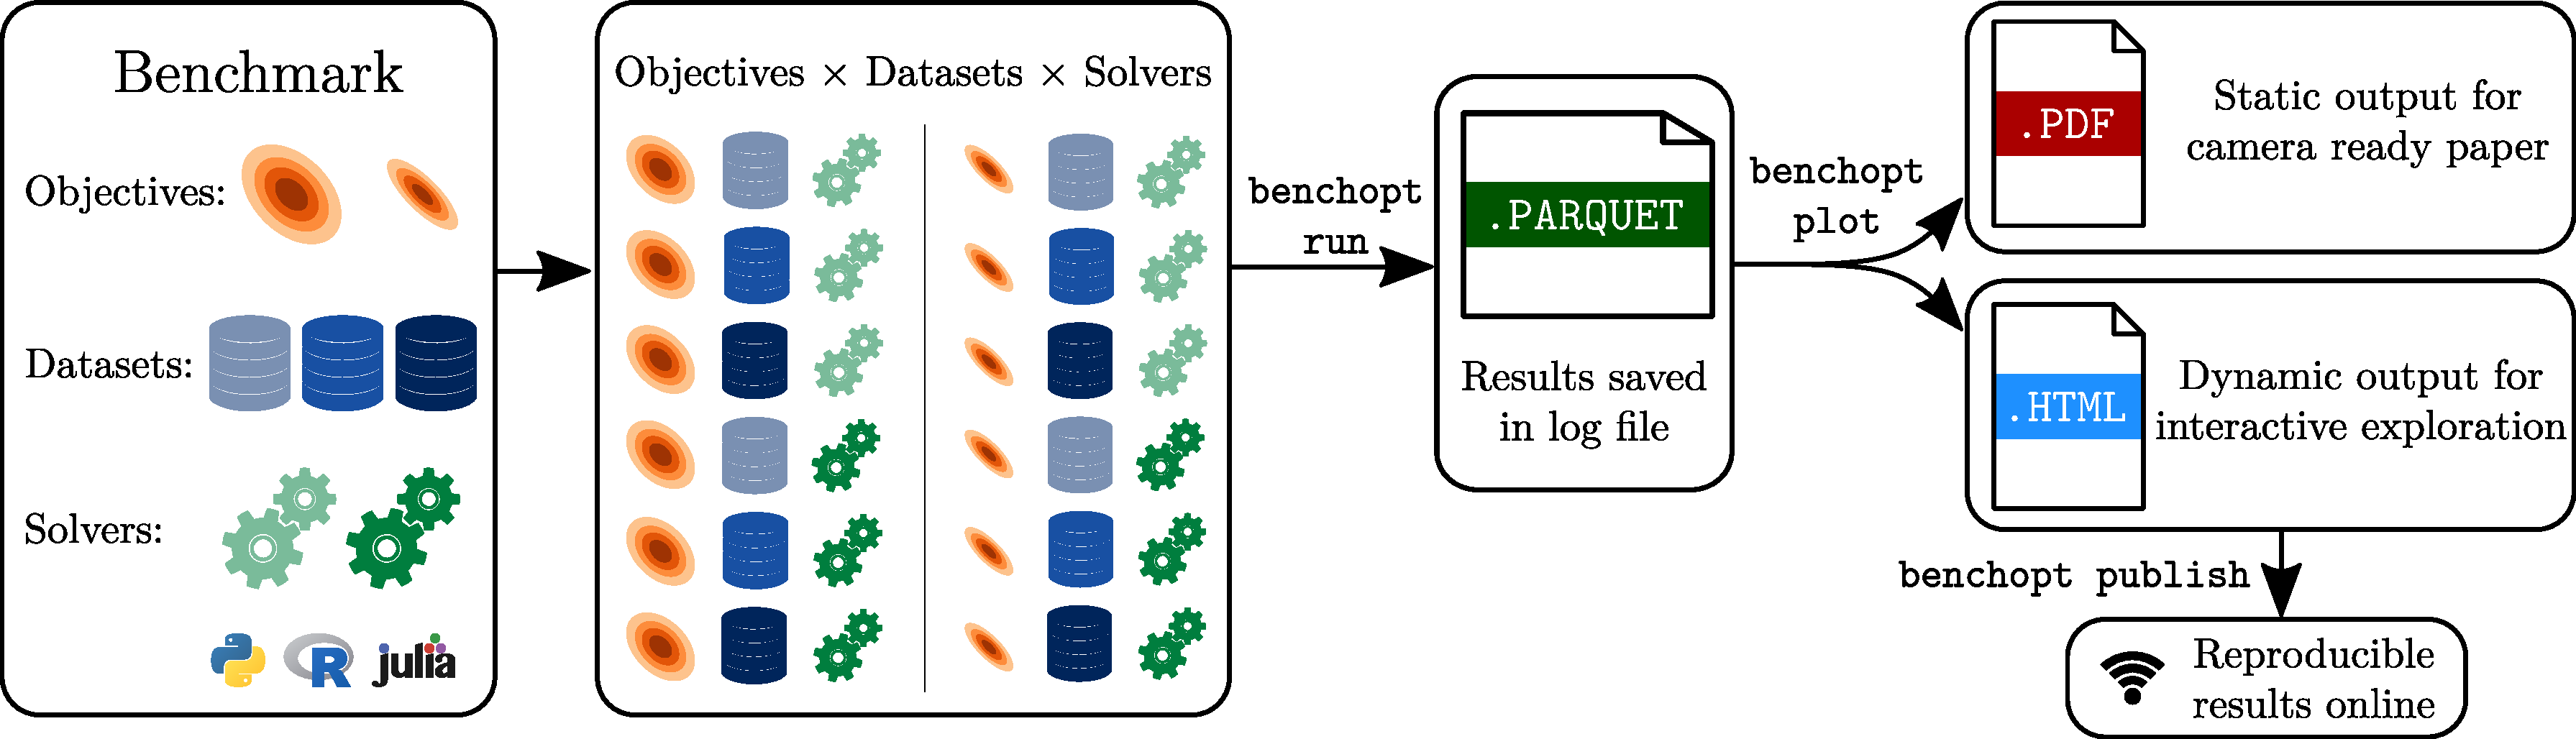
\includegraphics[width=\linewidth]{../sharedimages/benchopt_schema.pdf}

\end{frame}
%%%%%%%%%%%%%%%%%%%%%%%%%%%%%%%%%%%%%%%%%%%%%%%%%%%%%%%%%%%%%%%%%%%%%%%%%%%%%%%


%%%%%%%%%%%%%%%%%%%%%%%%%%%%%%%%%%%%%%%%%%%%%%%%%%%%%%%%%%%%%%%%%%%%%%%%%%%%%%%
\begin{frame}{Structure of a benchmark}

    \begin{minipage}{0.45\linewidth}
        \dirtree{%
        .1 benchmark/.
        .2 objective.py.
        .2 datasets/.
        .3 dataset1.py.
        .3 dataset2.py.
        .2 solvers/.
        .3 solver1.py.
        .3 solver2.py.
    }
    \end{minipage}

    Adding a solver? add a file

    Adding a dataset? add a file

\end{frame}
%%%%%%%%%%%%%%%%%%%%%%%%%%%%%%%%%%%%%%%%%%%%%%%%%%%%%%%%%%%%%%%%%%%%%%%%%%%%%%%

%%%%%%%%%%%%%%%%%%%%%%%%%%%%%%%%%%%%%%%%%%%%%%%%%%%%%%%%%%%%%%%%%%%%%%%%%%%%%%%
\begin{frame}{Running benchmarks + results}

    CSV, plotly for interactive exploration

    maybe merge with below
\end{frame}
%%%%%%%%%%%%%%%%%%%%%%%%%%%%%%%%%%%%%%%%%%%%%%%%%%%%%%%%%%%%%%%%%%%%%%%%%%%%%%%


%%%%%%%%%%%%%%%%%%%%%%%%%%%%%%%%%%%%%%%%%%%%%%%%%%%%%%%%%%%%%%%%%%%%%%%%%%%%%%%
\begin{frame}{\texttt{benchopt}}

    Metrics to follow, multiple parameters for a solver, easy way to filter out solvers

    HTML results are easy to share between collaborators, can be uploaded

    Parallel runs, results caching, csv
\end{frame}
%%%%%%%%%%%%%%%%%%%%%%%%%%%%%%%%%%%%%%%%%%%%%%%%%%%%%%%%%%%%%%%%%%%%%%%%%%%%%%%


%%%%%%%%%%%%%%%%%%%%%%%%%%%%%%%%%%%%%%%%%%%%%%%%%%%%%%%%%%%%%%%%%%%%%%%%%%%%%%%
\begin{frame}{Resnet benchmark}
    In the paper we present 10 benchmarks and in particular 3, resnets
\end{frame}
%%%%%%%%%%%%%%%%%%%%%%%%%%%%%%%%%%%%%%%%%%%%%%%%%%%%%%%%%%%%%%%%%%%%%%%%%%%%%%%




% %%%%%%%%%%%%%%%%%%%%%%%%%%%%%%%%%%%%%%%%%%%%%%%%%%%%%%%%%%%%%%%%%%%%%%%%%%%%%%%
% \begin{frame}{\texttt{benchopt}}
%     \centering
%     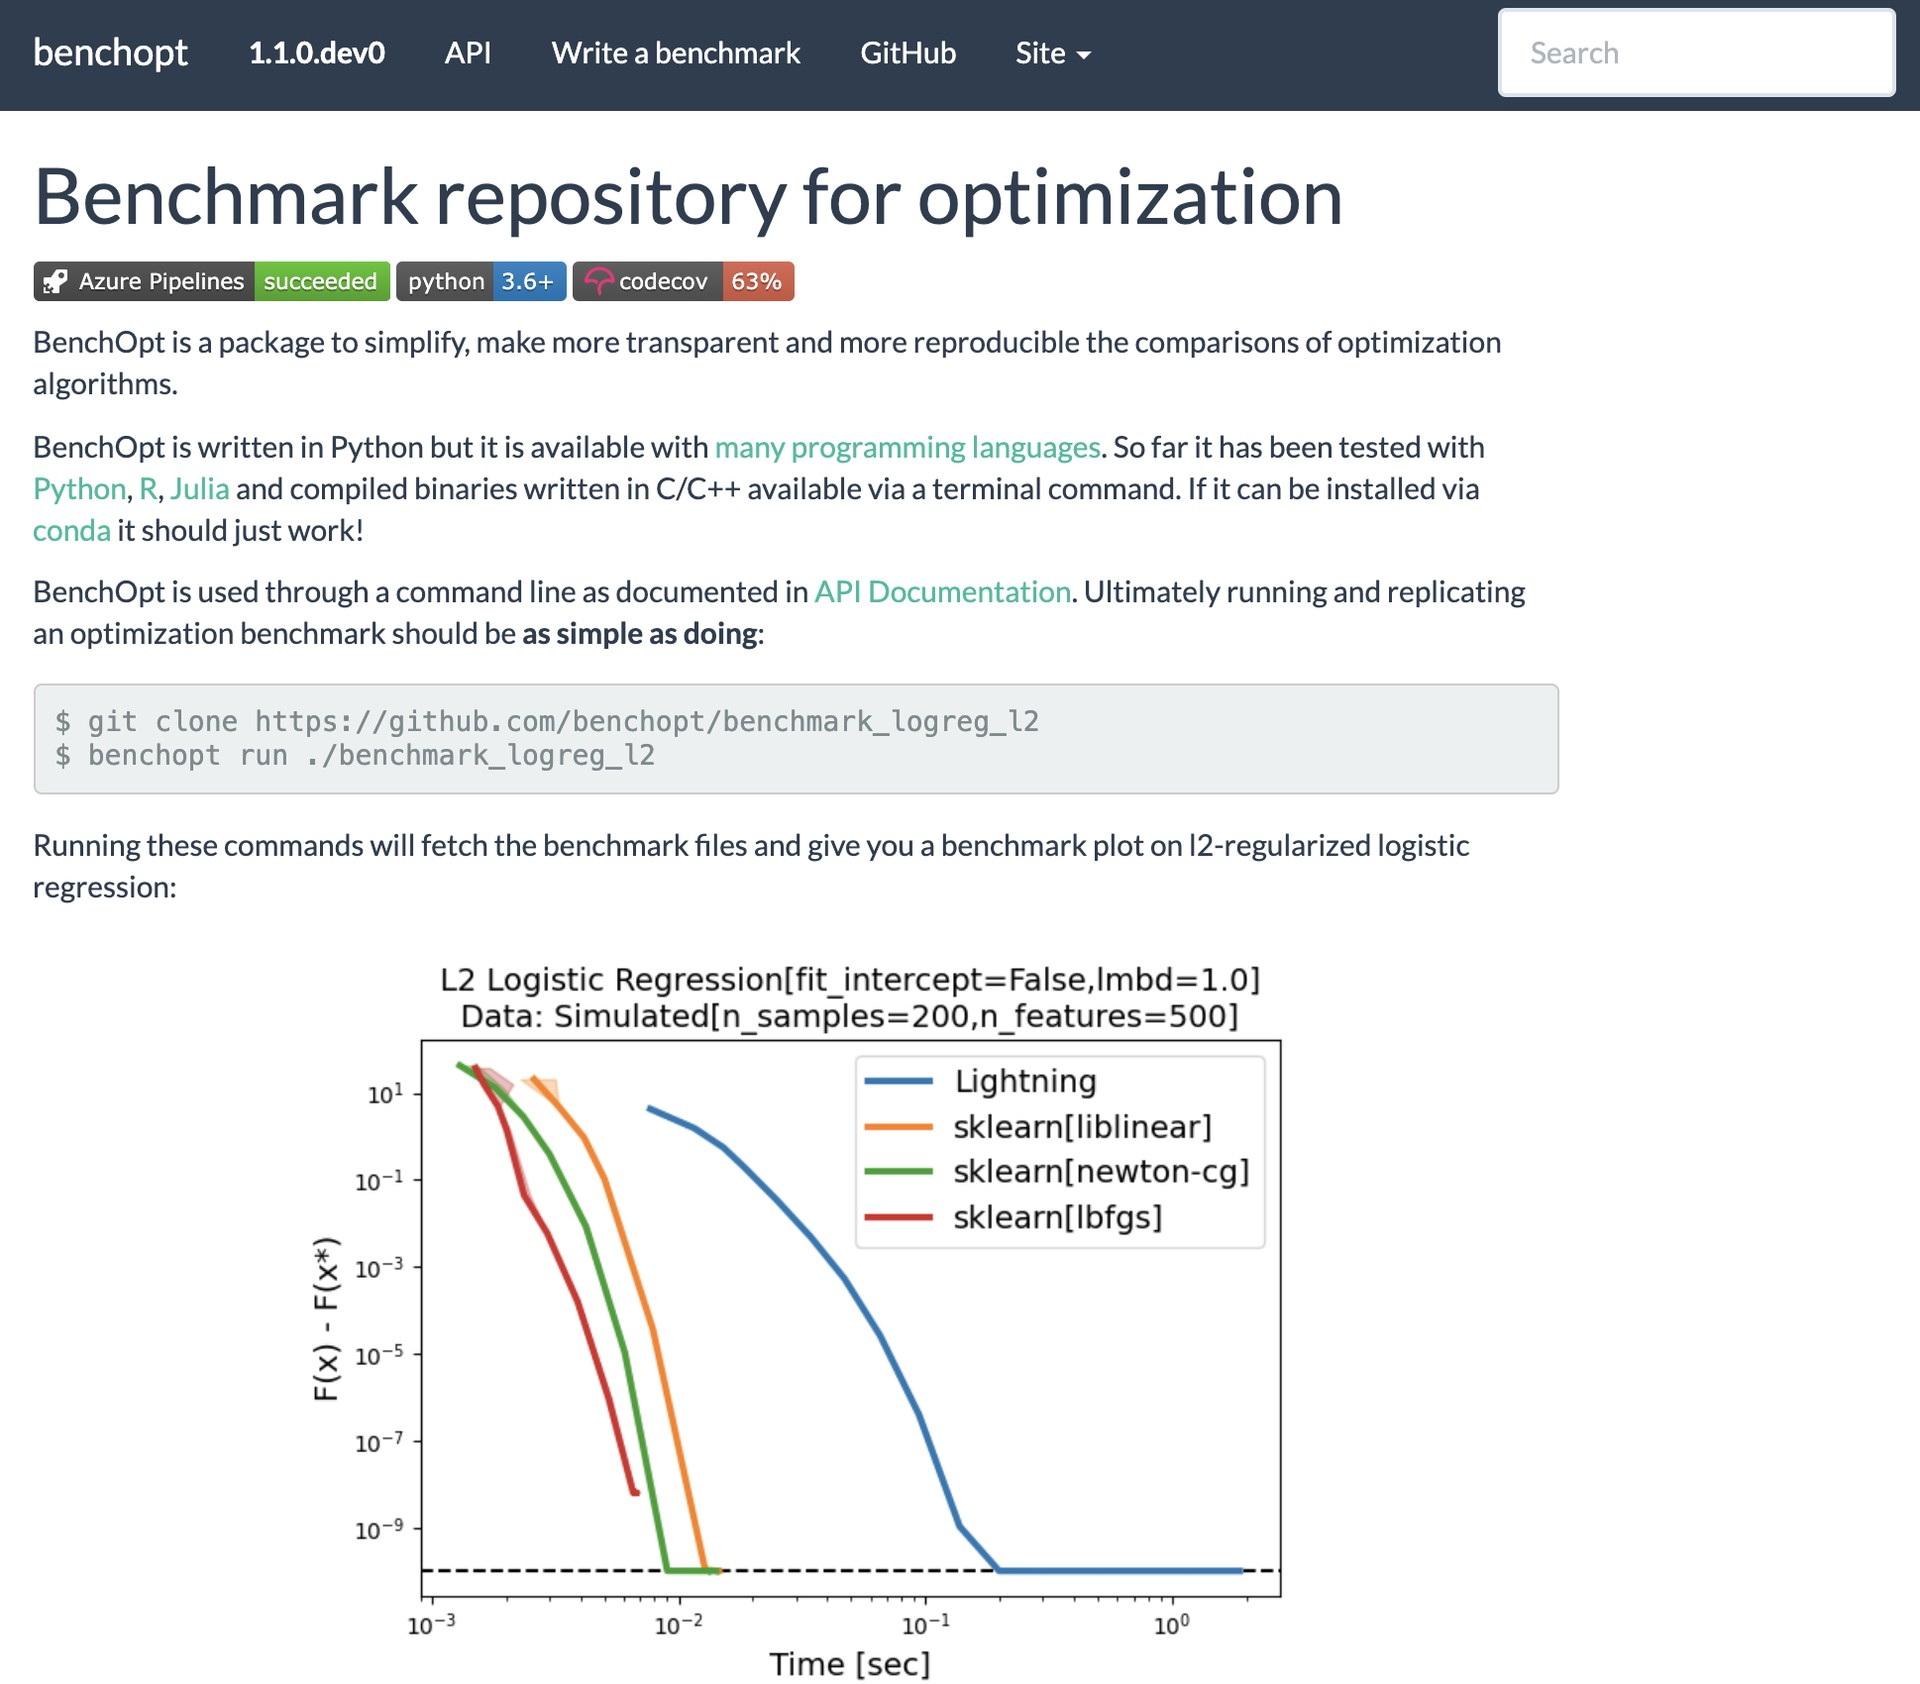
\includegraphics[width=.9\textwidth]{benchopt}\\
% \end{frame}
% %%%%%%%%%%%%%%%%%%%%%%%%%%%%%%%%%%%%%%%%%%%%%%%%%%%%%%%%%%%%%%%%%%%%%%%%%%%%%%%


% %%%%%%%%%%%%%%%%%%%%%%%%%%%%%%%%%%%%%%%%%%%%%%%%%%%%%%%%%%%%%%%%%%%%%%%%%%%%%%%
% \begin{frame}{Contact}

% \vspace{0.4cm}
% \centering
% \includegraphics[width=0.93\textwidth]{contact_js}
% \end{frame}
% %%%%%%%%%%%%%%%%%%%%%%%%%%%%%%%%%%%%%%%%%%%%%%%%%%%%%%%%%%%%%%%%%%%%%%%%%%%%%%%



% %%%%%%%%%%%%%%%%%%%%%%%%%%%%%%%%%%%%%%%%%%%%%%%%%%%%%%%%%%%%%%%%%%%%%%%%%%%%%%%
% % Uncomment for references
% \begin{frame}{Bibliographie}
% \printbibliography
% \end{frame}
%  %%%%%%%%%%%%%%%%%%%%%%%%%%%%%%%%%%%%%%%%%%%%%%%%%%%%%%%%%%%%%%%%%%%%%%%%%%%%%%



\end{document}
